\documentclass[conference]{IEEEtran}
\IEEEoverridecommandlockouts
% The preceding line is only needed to identify funding in the first footnote. If that is unneeded, please comment it out.
\usepackage{cite}
\usepackage{amsmath,amssymb,amsfonts}
\usepackage{algorithmic}
\usepackage{graphicx}
\usepackage{textcomp}
\usepackage{xcolor}
\def\BibTeX{{\rm B\kern-.05em{\sc i\kern-.025em b}\kern-.08em
    T\kern-.1667em\lower.7ex\hbox{E}\kern-.125emX}}
\usepackage{listings}
\lstset{
  frame=single,
  language=python,
  basicstyle=\small,
}

\makeatletter
\def\lst@makecaption{%
  \def\@captype{table}%
  \@makecaption
}
\makeatother

\begin{document}

\title{Benchmarking Agents Across Diverse Tasks}

\author{
\IEEEauthorblockN{Alexander Moore}
\IEEEauthorblockA{\textit{Data Science} \\
\textit{Worcester Polytechnic Institute}\\
Worcester, United States \\
ammoore@wpi.edu}

\and

\IEEEauthorblockN{Brian Lewandowski}
\IEEEauthorblockA{\textit{Computer Science} \\
\textit{Worcester Polytechnic Institute}\\
Worcester, United States \\
balewandowski@wpi.edu}

\and

\IEEEauthorblockN{Jannik Haas}
\IEEEauthorblockA{\textit{Data Science} \\
\textit{Worcester Polytechnic Institute}\\
Worcester, United States \\
jbhaas@wpi.edu}

\and

\IEEEauthorblockN{Quincy Hershey}
\IEEEauthorblockA{\textit{Data Science} \\
\textit{Worcester Polytechnic Institute}\\
Worcester, United States \\
qbhershey@wpi.edu}

\and

\IEEEauthorblockN{Scott Tang}
\IEEEauthorblockA{\textit{Data Science} \\
\textit{Worcester Polytechnic Institute}\\
Worcester, United States \\
stang3@wpi.edu}
}

\maketitle

\begin{abstract}
    Understanding which models succeed (and why) at which tasks is a foundational experience in reinforcement learning.
    Following a baseline of techniques and best practices found in the literature this project will show a comparison of multiple reinforcement learning techniques applied in a few common environments.
    In particular, this project implements several algorithms under the Q-learning, policy learning, and actor-critic categories and compares the results across several tasks.
    It is shown where these algorithms work strongly on some tasks and perform poorly on others.
    This work explores a set of baseline results for diverse reinforcement learning algorithms, in order to compare and contrast the performance of models on diverse tasks.
\end{abstract}

\begin{IEEEkeywords}
Q-Learning, Policy Learning, DQN, Policy Gradient, actor-critic, Reinforcement Learning
\end{IEEEkeywords}

\section{Introduction}
Project 3 explored how to construct a Deep Q Network (DQN) by following the classic DQN algorithm outlined originally in \cite{DQNOriginalPaper}.
Building off of this recent experience this project takes the deep learning techniques discussed in class and applies them to several well-known tasks using Q-learning, policy learning, and actor-critic methods.
The results of these methods are compared and discussed.

The openai gym \footnote{https://gym.openai.com/} was chosen to be used as the game environment.
Two games were chosen to be used for comparison of the algorithms in this paper.
First, the Breakout game was used for its familiarity from Project 3 and that it has a known level of difficulty.
In addition, it serves as a discrete action space environment.
To contrast with this, the MountainCar was also chosen as it has both a discrete and continuous action space environment available for use.
Using these environments multiple agents were trained and tested using DQN, Double DQN, Dueling DQN, REINFORCE, Proximal Policy Optimization (PPO), and Advantage Actor Critic (A2C).
This work shows that these algorithms all have strengths and weaknesses in a wide variety of areas including task completion, complexity, training time, and sensitivity to hyperparameters.

The remainder of this paper is organized as follows:
\begin{itemize}
\item Section \ref{background} provides background information regarding the methods implemented.
\item Section \ref{methodology} provides a description of the methodology used to train, execute, and assess the algorithms explored.
\item Section \ref{results} provides a discussion of the training process and associated results.
\item Finally, the paper concludes in section \ref{conclusion}.
\end{itemize}

\section{Background Information} \label{background}

\subsection{Deep Q Learning}
Deep Q learning uses a deep neural network to learn coefficients $\omega$ such that the network's value function evaluates $(state, action)$ pairs improving the model's task reward. For some of our environments this will be a convolution over a screen space, and for some we might extract some derived features about the game for the model to use as a state representation.

\subsection{Double Deep Q Learning}
Double deep Q networks address the maximization bias problem from Deep q learning by instead letting two Q functions randomly select the action and update the corresponding Q function. This process inhibits bias and will potentially converge faster or outright outperform DQN on all tasks.

\subsection{Dueling Deep Q Learning}
Dueling DQN separates the Q-learning process into two functions, the sum of the state and state-action estimator models. This approach ideally learns how to relatively value states by accounting for a learned state-value function $V(s)$, as well as an advantage function $A(s,a)$ interpreted as the value of taking action $a$ while in state $s$. For this reason this different approach will be interesting to analyze on tasks where the actions might not always directly affect the environment, for example in breakout where many movements have no direct affect on the game environment.

\subsection{Basic Policy Gradient}
Policy gradient algorithms in general are methods that learn a parameterized policy that can select actions without consulting a value function \cite{ReinforcementLearningBook}.
A value function may be utilized or learned to support learning a given policy, however, it is not involved in the process of choosing an action with these methods \cite{ReinforcementLearningBook}.
The Basic Policy Gradient algorithm treats learning of the policy as an episodic case using a performance measure that equates to the reward obtained following the current policy given a starting state of an episode. 
At its core, the Basic Policy Gradient algorithm takes the gradient of expected rewards for an episode and uses it to update the policy parameters.
This can be summarized by the two equations below,

$$\nabla \bar{R}_{\theta} = \frac{1}{N} \sum \limits_{n=1}^N \sum \limits_{t=1}^{T_n} R(\tau^n) \nabla log\pi_{\theta}(a_{t}^n | s_{t}^n)$$

$$\theta = \theta  + \eta \nabla \bar{R}_{\theta}$$

where N is the number of episodes, T is the steps within an episode, R is the reward for a given episode, $\theta$ are the policy parameters, a is a given action, and s is a given state.

Implemented in pseudocode, this algorithm would be similar to Listing \ref{listing:basicPolicyGradientAlg}.
While not implemented as part of this project is is the building block for all subsequently developed policy gradient models.

\begin{lstlisting}[
    float=t,
    caption=\textbf{Basic Policy Gradient} The basic policy gradient algorithm,
    label=listing:basicPolicyGradientAlg,
]

Loop until stopping criteria met:
    for a batch of episodes:
        - Step through episode
        - Store reward gained

    - Determine reward gradient of batch
    - Update policy parameters
\end{lstlisting}

\subsection{REINFORCE Policy Gradient}
The REINFORCE Policy Gradient method also referred to as Monte-Carlo Policy Gradient makes a slight adjustment to the Basic Policy Gradient algorithm of using the return from each time step instead of the overall reward from the episode in the update of the policy parameters. This will reduce the high variance of the standard basic policy gradient algorithm.
This change can be seen in the pseudocode in Listing \ref{listing:reinforcePolicyGradientAlg}. 

\begin{lstlisting}[
    float=h,
    mathescape = true
    caption=\textbf{REINFORCE Policy Gradient} The reinforce policy gradient algorithm,
    label=listing:reinforcePolicyGradientAlg,
]

For each episode from the current policy:
    For t=1 to T-1 do:
        {$\theta = \theta  + \alpha \nabla_{\theta} log\pi_{\theta}(s_t, a_t)G_t$}

    end for
end for
return {$\theta$}
\end{lstlisting}

\subsection{PPO Policy Gradient}
Unlike the Basic and REINFORCE policy gradient algorithms, the Proximal Policy Optimization (PPO) algorithm is an off-policy method, where the performance assessment and improvement of a policy is different than the one used for action selection (or sampling). The separate policies allow the collected data to be used more than once, which result in faster performance. PPO also addresses other shortcomings of the Basic Policy Gradient by subtracting the state-value off as the baseline to improve update accuracy when rewards are non-negative via an Advantage function. This function also serves to reduce large variance without increasing bias. Finally, PPO improves stability by imposing a constraint on the distance (or difference) between the old and new policies by clipping their ratio to a small interval around one.

\subsection{Advantage Actor Critic}
Actor-Critic methods, similar to the REINFORCE algorithm, learn both a policy function and state-value function.
The main difference between them, however, is the fact that actor-critic methods use the value function as a way to bootstrap the value estimation.
The implementation for this work follows closely to the "One-step Actor-Critic" algorithm outlined in \cite{ReinforcementLearningBook} with some practical updates for implementation.
It is a temporal difference algorithm that relies solely on the current step for learning.
This is in contrast to the many of the other algorithms implemented in this work as they involve utilizing a replay buffer for batch learning.

In addition, it should be noted that this implementation remains a basic implementation and does not include the commonly seen updates added to this method such as an additional entropy loss.

\section{Methodology} \label{methodology}

\subsection{Tools and Framework}
This project used the Python language and several python libraries. 
In addition to the standard libraries, the following additional libraries were used:
 
\begin{itemize}
    \item OpenAI Gym \cite{openaigym}
    \item PyTorch
    \item NumPy
    \item Matplotlib
    \item Pandas
\end{itemize}

The framework provided from Project 3 was built off of and adapted to support additional environments aside from Breakout.
A framework was built such that the main training and testing pipeline was consistent across algorithm implementations.
This allowed for each team member to focus on implementing specific models and algorithm learning details.

The general workflow using this framework can be seen in Listing \ref{listing:basicModelWorkflow}.

\begin{lstlisting}[
    float=t,
    caption=\textbf{Algorithm Development Workflow} The basic workflow used to develop new models and algorithms.,
    label=listing:basicModelWorkflow,
]

# Create a new model in models directory
# - Implement the __init__ function
# - Implement the forward function

# Create a new agent in the agents directory
# - Implement the make_action function
# - Implement the can_train function
# - Implement the train function

# Execute training for model on command line
# python main.py \
#    --train_dqn \
#    --model sample_model.SampleModel \
#    --agent sample_agent.SampleAgent \
#    --other_arguments

\end{lstlisting}

It should be noted that all agents inherit a set of functions from a base class allowing for a small barrier to entry in setting up new agents.
An agent runner class was constructed such that it handles the main training loop used by all algorithms implemented while the learning details are held within the specific agents themselves.

In addition, during model training, this framework stores all arguments used to start the session as well as periodic interim models and statistics in both raw format and as plots.
This allowed for repeatability and easy metrics collection during every session.
An example view of what this archive directory looks like can be seen in Listing \ref{listing:sampleModelArchive}.

\begin{lstlisting}[
    float=t,
    caption=\textbf{Model Training Archive} A typical archive from a model that has been trained for 2000 episodes.,
    label=listing:sampleModelArchive,
]

archive/
   |
   test_learning_rate/
       |
       args.pkl
       1000_model.pth
       1000_optimizer.pth
       1000_training_metrics.csv
       1000_training_reward_plot.png
       1000_test_metrics.csv
       1000_test_reward_plot.png
       2000_model.pth
       2000_optimizer.pth
       2000_training_metrics.csv
       2000_training_reward_plot.png
       2000_test_metrics.csv
       2000_test_reward_plot.png
\end{lstlisting}

\subsection{Gym Environments}
Several different environments from the openai gym python packages were utilized on this project.
A description of each of these environments and a description of the task to be solved by agents within them follows.

\subsubsection{BreakoutNoFrameskip-v4}
The Breakout environment involves interacting with the Atari 2600 game by the agent receiving image data for what has been seen on screen.
After pre-processing handled by the atari wrapper code the state space consists of 4 stacked 84x84 images.
The action space for this environment consists of 4 possible discrete actions:

\begin{itemize}
    \item LEFT - Move agent left
    \item RIGHT - Move agent right
    \item NOOP - Do nothing
    \item FIRE - Places ball in motion at start of new lives
\end{itemize}

This environment was chosen as it was familiar from Project 3 and sufficiently difficult for naive models.
In addition, it serves as a well-contained discrete action space for all algorithms under test.

The reward structure for this environment consists of the traditional values for the blocks in the game where the first two levels provide one point, the next two levels provide 3 points, and the final two levels provide 7 points.
For the learning agent, the atari wrapper environment clips this reward to be just one point for a timestep where a brick was broken.

\subsubsection{MountainCarContinuous-v0}
The Mountain Car environment in both its original and continuous form consists of the agent being a car beginning in the valley between two mountains.
In this classic control task, the agent must apply a specific force to the mountain car with the goal of reaching the top of the right hand mountain as seen by the flag in Figure \ref{fig:mountainCarEnvironment}.

\begin{figure}[htbp]
\centerline{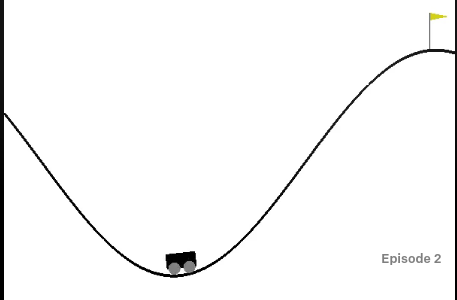
\includegraphics[scale=0.5]{mountain_car.png}}
\caption{\textbf{Example of the Mountain Car Environment}  The mountain car environment provided by openai.}
\label{fig:mountainCarEnvironment}
\end{figure}

In this environment, the agent must learn to gather enough momentum by first going backwards a bit prior to going forwards in order to have enough acceleration to reach the flag.

The state space for this environment consists only of the mountain car's position and velocity.
The action space for this environment is a single continuous action which is the force to be applied to the mountain car.
A positive value is a force towards the goal and a negative value for this force puts the mountain car in reverse.

The reward structure for this environment consists of the agent receiving a small negative reward for the number of actions taken and a positive reward of 100 when reaching the goal.
This environment is considered solved once a score of 90 is achieved \footnote{https://github.com/openai/gym/wiki/MountainCarContinuous-v0}.

This environment was chosen as it is a well-suited introductory environment to explore continuous action spaces.

\subsubsection{MountainCar-v0}
The MountainCar-v0 environment is the discrete action-space relative of MountainCarContinuous-v0 as described above.
This environment entails the same general principles and overall goal but the action space has been altered to use discrete actions as listed below.

\begin{itemize}
    \item PUSH LEFT
    \item PUSH RIGHT
    \item NO PUSH
\end{itemize}

The state-space for this environment remains unchanged.
The reward structure for this environment consists of -1 for each time step until the goal is reached.
The environment is considered solved if an average of -110 points is achieved over 100 consecutive trials \footnote{https://github.com/openai/gym/wiki/MountainCar-v0}.

\subsection{Continuous Action Spaces}
One of the key goals for this project was to interact in an environment with continuous action spaces.
In general, models that operate in discrete action spaces take as input the state space (or state-space and action) and return either a value function or policy function.
The value function represents the value of the particular state and the policy function generally provides an action or probabilities for which actions to execute.

When dealing with continuous action spaces, this is shifted such that the policy learned is the mean and standard deviation for desirable actions within a continuous action space.
As the agent learns, the standard deviation generally starts out wide and then narrows once it is more confident in the actions to take.
Choosing an action consists of sampling from the learned distribution.

\subsection{Continuous Advantage Actor Critic Implementation}
The actor critic implementation follows closely to the "One-step Actor-Critic" algorithm outlined in \cite{ReinforcementLearningBook} with some practical updates made for implementation adapted from Phil Tabor's public codebase \footnote{https://github.com/philtabor}.
This implementation is a temporal difference algorithm using no replay buffer and using only the current time step information to facilitate learning.
In addition, it is implemented in an on-policy manner.

The target for this model was the MountainCarContinuous-v0 environment so the model and agent were structured with this in mind.
One can see the model structure and hyperparameters of the final model in Listing \ref{listing:continuousActorCriticModel} and Table \ref{table:continuousActorCriticHypers} respectively.


\begin{lstlisting}[
  float=t,
  caption=\textbf{Continuous Actor Critic Model}  The model architecture used for the continuous actor critic implementation.,
  label=listing:continuousActorCriticModel,
]
Fully Connected:   2 Input,512 Output
ReLU

|
v

Fully Connected:  512 Input, 512 Output  
ReLU

|\
| \
|  \
|   |
|   v
|  Value Output Layer:  512 Input; 1 Output
|
v

Policy Mean 
Output Layer:   512 Input;  1 Output
tanh

Policy Standard Deviation 
Output Layer:  512 Input;  1 Output
Softplus
\end{lstlisting}

\begin{table}[htbp]
    \caption{\textbf{Continuous Advantage Actor Critic Hyperparameters}  The hyperparameters used for training the continuous actor critic agent.}
\begin{center}
\begin{tabular}{|c|c|c|}
\hline
\textbf{Hyperparameter} & \textbf{Value} \\
\hline
\textbf{Batch Size} & Does not apply \\
\hline
\textbf{Learning Rate} & 0.00015 \\
\hline
\textbf{Replay Buffer Size} & Does not apply \\
\hline
\textbf{Minimum Buffer Training Size} & Does not apply \\
\hline
\textbf{Starting Epsilon} & Does not apply \\
\hline
\textbf{Final Epsilon} & Does not apply \\
\hline
\textbf{Epsilon Decay Steps} & Does not apply \\
\hline
\textbf{Gamma} & 0.99\\
\hline
\textbf{Loss Function} &  -log\_loss * advantage \\
\hline
\textbf{Optimizer} & Adam \\
\hline
\textbf{Target Network Update Interval} & Does not apply \\
\hline
\end{tabular}
\label{table:continuousActorCriticHypers}
\end{center}
\end{table}


\subsection{Discrete Advantage Actor Critic Implementation}
The discrete version of the actor critic algorithm adapted the continuous version discussed earlier for the BreakoutNoFrameskip-v4 environment.
This included incorporating a known model baseline previously shown effective in this environment while adapting it for returning both the policy and values necessary for the actor critic method.

The model structure and hyperparameters for this implementation can be seen in Listing \ref{listing:discreteActorCriticModel} and Table \ref{table:discreteActorCriticHypers} respectively.

\begin{lstlisting}[
  float=t,
  caption=\textbf{Discrete Actor Critic Model}  The model architecture used for the discrete actor critic implementation.,
  label=listing:discreteActorCriticModel,
]
CNN:  32 8x8 filters, stride 4
ReLU

|
v

CNN:  64 4x4 filters, stride 2
ReLU

|
v

CNN:  64 3x3 filters, stride 1
ReLU

|
v

Fully Connected: 3136 Input; 512 Output
ReLU

|\
| \
|  \
|   |
|   v
|  Value Output Layer:  512 Input; 1 Output
|
v

Policy Output Layer: 512 Input;  4 Output
SoftMax
\end{lstlisting}

\begin{table}[htbp]
    \caption{\textbf{Discrete Advantage Actor Critic Hyperparameters}  The hyperparameters used for training the discrete actor critic agent.}
\begin{center}
\begin{tabular}{|c|c|c|}
\hline
\textbf{Hyperparameter} & \textbf{Value} \\
\hline
\textbf{Batch Size} & Does not apply \\
\hline
\textbf{Learning Rate} & 0.0003\\
\hline
\textbf{Replay Buffer Size} & Does not apply \\
\hline
\textbf{Minimum Buffer Training Size} & Does not apply \\
\hline
\textbf{Starting Epsilon} & Does not apply \\
\hline
\textbf{Final Epsilon} & Does not apply \\
\hline
\textbf{Epsilon Decay Steps} & Does not apply \\
\hline
\textbf{Gamma} & 0.99\\
\hline
\textbf{Loss Function} &  -log\_loss * advantage \\
\hline
\textbf{Optimizer} & Adam \\
\hline
\textbf{Target Network Update Interval} & Does not apply \\
\hline
\end{tabular}
\label{table:discreteActorCriticHypers}
\end{center}
\end{table}

\section{Results} \label{results}

\subsection{Continuous Advantage Actor Critic}

\subsection{Discrete Advantage Actor Critic}

\section{Planned Work} \label{planned}

\section{Conclusion} \label{conclusion}
Here, there should be an in-depth discussion about the way each model performed on each task and how those findings either agree or disagree with our expectations and hypotheses about the models, tasks, agents, and parameters.

This project represents an approximate survey of diverse models from the Reinforcement Learning course, as well as the challenges and benefits of implementation of these methods on very different tasks. The project goal was effectively a combination of 6 models across 2 tasks, taking for 12 applications of a Project-3-like assignment. However, instead of simply doing 12 unique projects, this group wanted to emphasize the contrast in application between these different models on these different tasks.

Among the time-expensive nature of training many agents on multiple tasks, our largest efforts were in the development of so many different models. These difficulties were effectively 6-8 project three development times, as we split the agent development among team members. In hindsight, in order to better address the goals of this project, we would make some changes to the experimental design and workflow of the project. Having a shared `agent\_runner` was a huge benefit, but instead of using that common core to develop many diverse agents, it is possible we could better address the goals of the experiment by using fewer models and more tasks. This change would give a better sense of the \_\_benchmarking\_\_ goal, as it would be interesting to compare some kind of human-performance normalized results of a handful of agents (DQN, policy gradient,) on many tasks, such as every atari game. As it stands, the deployment of more agents is an interesting comparison on a small number of tasks, but most of our resources went into the development of these diverse agents, as opposed to truly optimizing and benchmarking them. Another option to ameliorate these difficulties would be to rely only on other researcher's implementations of these algorithms, so that our group could focus on applying them and getting as many results as possible, instead of troubleshooting and programming.

\bibliography{citations.bib}{}
\bibliographystyle{plain}

\vspace{12pt}

\end{document}
